\mysubsubsectionformatted{Il Pattern architetturale "Layers"}
\myparagraph{
    Questo pattern permette di risolvere i problemi elencati in precedenza tramite l'uso dei layers.
    \\
    Un \textbf{\coloredtext[blue]{Layer}} è un elemento di grandi dimensioni, spesso composto da molti\\ package e sottosistemi.
    \begin{tcolorbox}[colback=blue!5!white, colframe=blue!75!black]
        Il pattern permette di organizzare l'architettura logica in un sistema a più livelli (layers) che
        comprendono funzionalità distinte ma correlate in modo da permettere una netta separazione delle responsabilità
        e un aumento della coesione del sistema stesso.
        \\
        I livelli più bassi comprendono i servizi più generali e di basso livello, quelli in alto saranno più specifici
        per la singola applicazione.
    \end{tcolorbox}
    \noindent Il numero di layer e il loro scopo non è fisso, cambia a seconda delle applicazioni. Ciascun layer si appoggia alle
    funzionalità dei layer sottostanti, ma possono comunicare anche con i layer di livelli più bassi. Ovviamente, come il sistema stesso,
    anche l'architettura a layer viene sviluppata in modo iterativo, l'obiettivo è quello di avere
    l'architettura fondamentale stabilita.
    \newpage
    \subsubsection{Esempio di architettura a layers}
    \begin{center}
        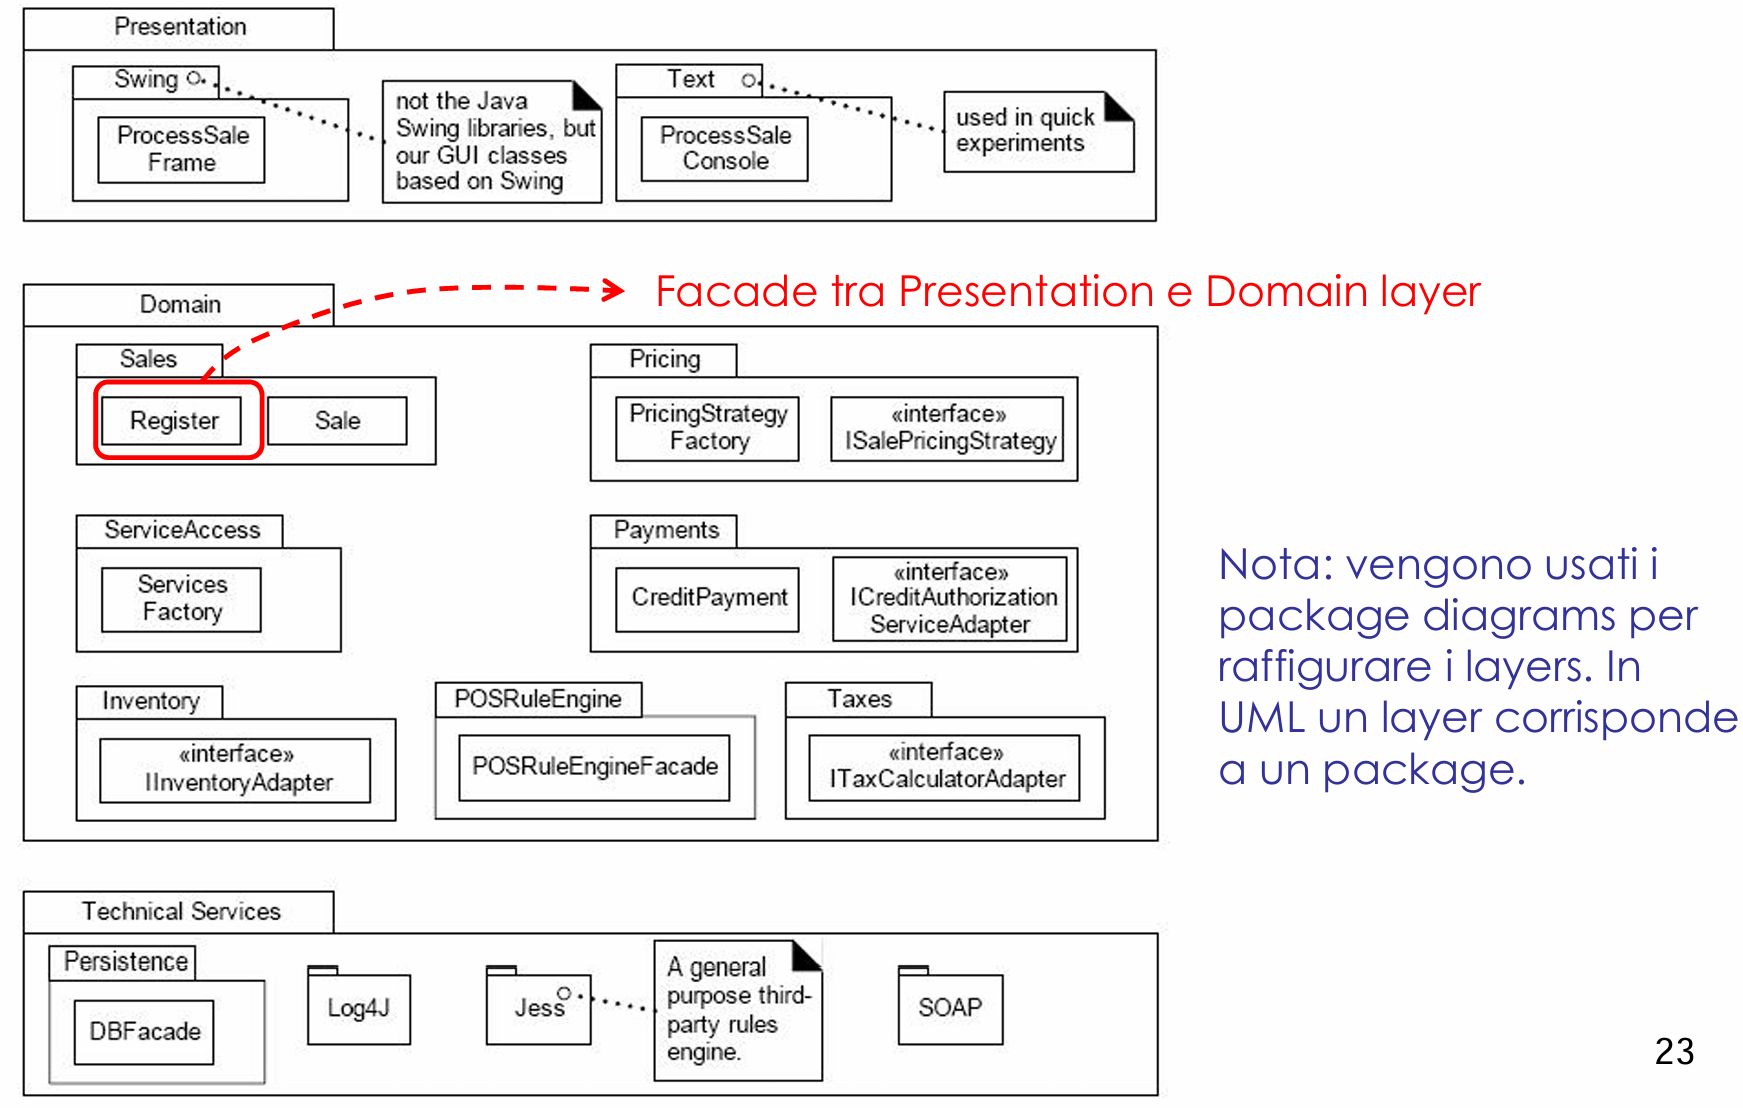
\includegraphics[scale=0.27]{architettura_layer/archi_layer_esempio.png}
    \end{center}
    \mysubsubsectionformatted{Considerazioni sull'Application Layer}
    \begin{itemize}
        \item Per conoscere lo stato del client si fa uso dei package Presentation e Domain. I due package collaborano tra loro
              per controllare il flusso di lavoro (l'ordine delle finestre, le pagine web\dots)
        \item L'Application Layer viene usato quando:
              \begin{enumerate}
                  \item Sono disponibili più interfacce utente. In questo caso vengono usati degli Adapter per collezionare i dati delle varie
                        interfacce e le Facade per nascondere l'accesso al Domain.
                  \item Il sistema è distribuito e il Domain si trova su un nodo diverso rispetto al Presentation.
                  \item Il Domain non può mantenere lo stato delle sessioni.
                  \item Esiste un workflow ben definito da seguire nella presentazione delle varie schermate.
              \end{enumerate}
    \end{itemize}
    \newpage
    \noindent Ovviamente esisteranno accoppiamenti fra i vari livelli, ma si possono raffigurare i più significativi
    attraverso un apposito diagramma.
    \begin{center}
        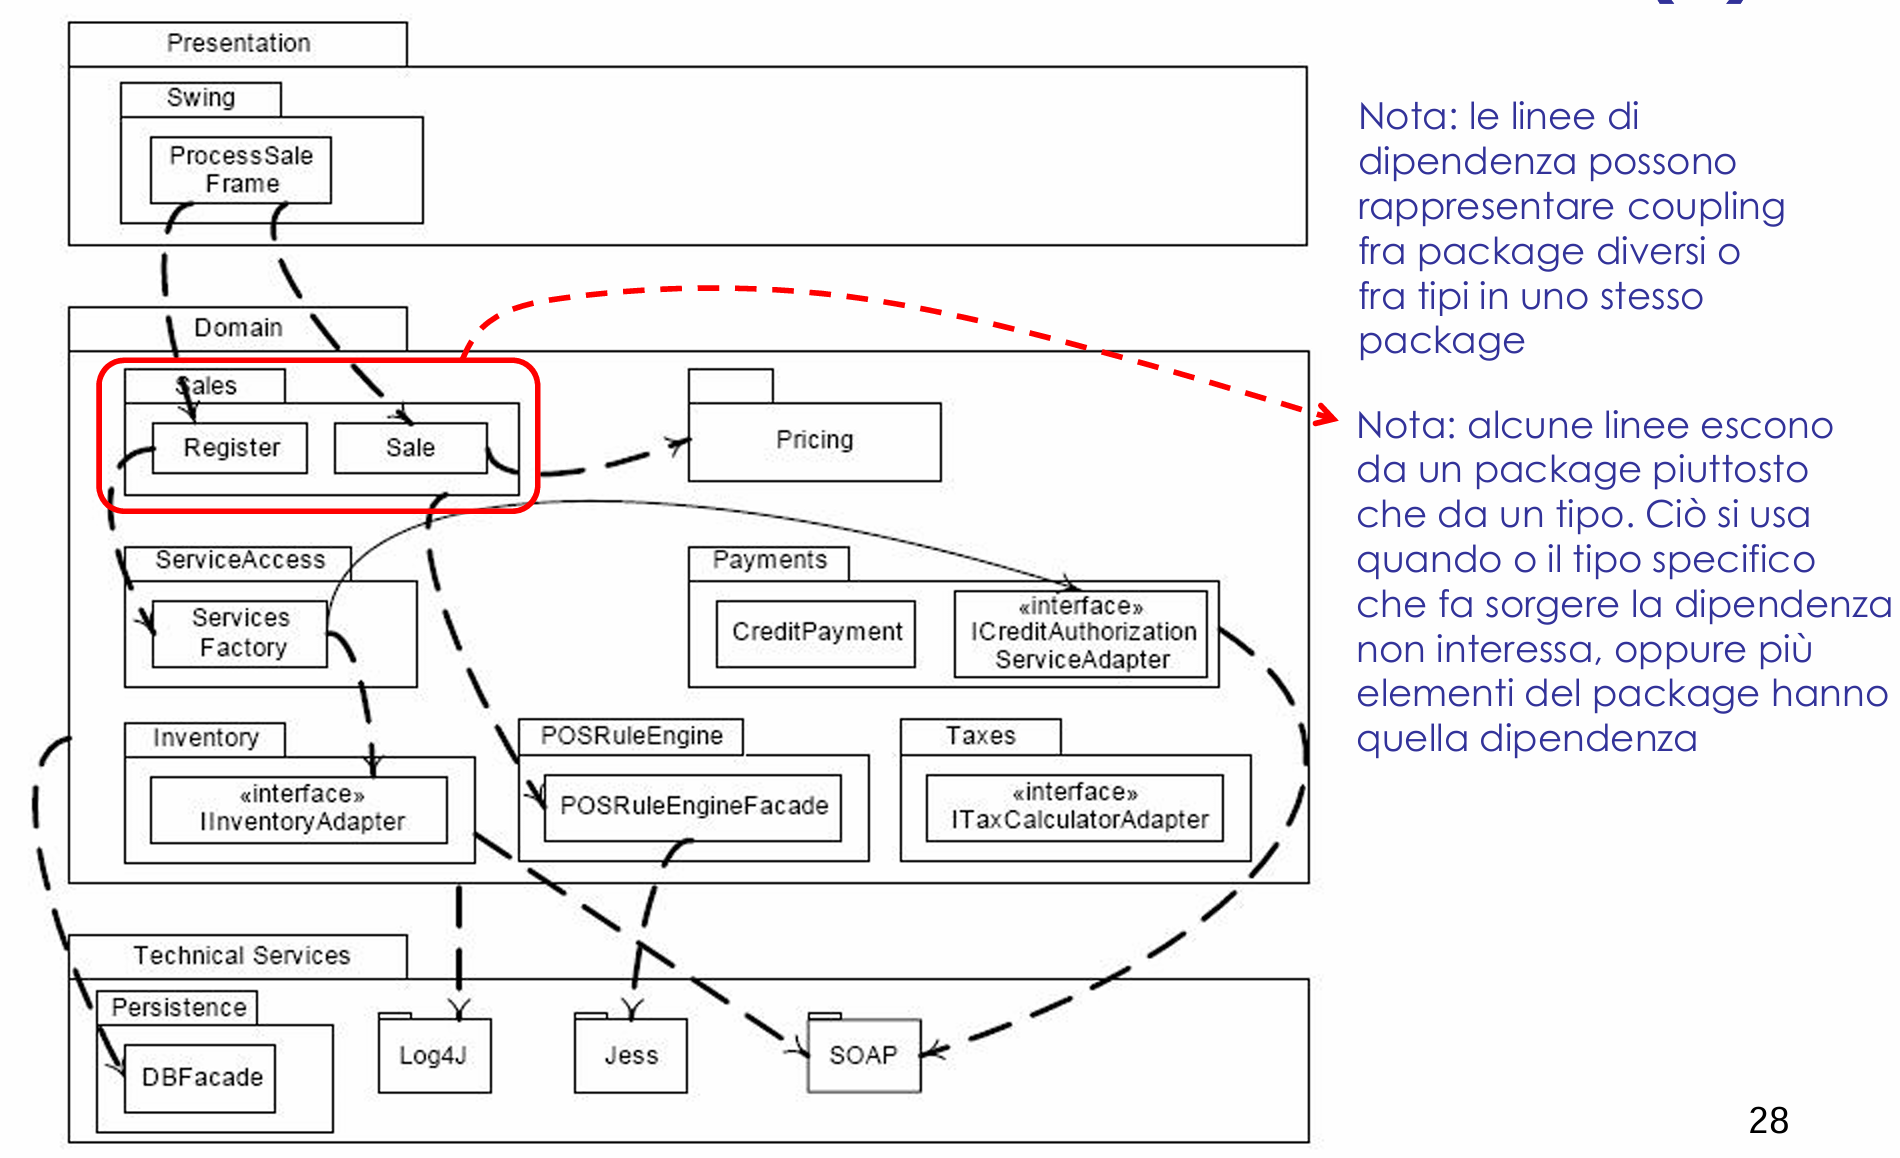
\includegraphics[scale=0.25]{architettura_layer/archi_layer_accoppiamenti.png}
    \end{center}
    Per capire meglio come gli oggetti fra i vari layer comunicano fra di loro si possono usare i \textbf{Diagrammi di Sequenza} in
    modo da rappresentare gli scenari architetturali più significativi.
    \subsubsection{Esempio di diagramma di sequenza}
    \begin{center}
        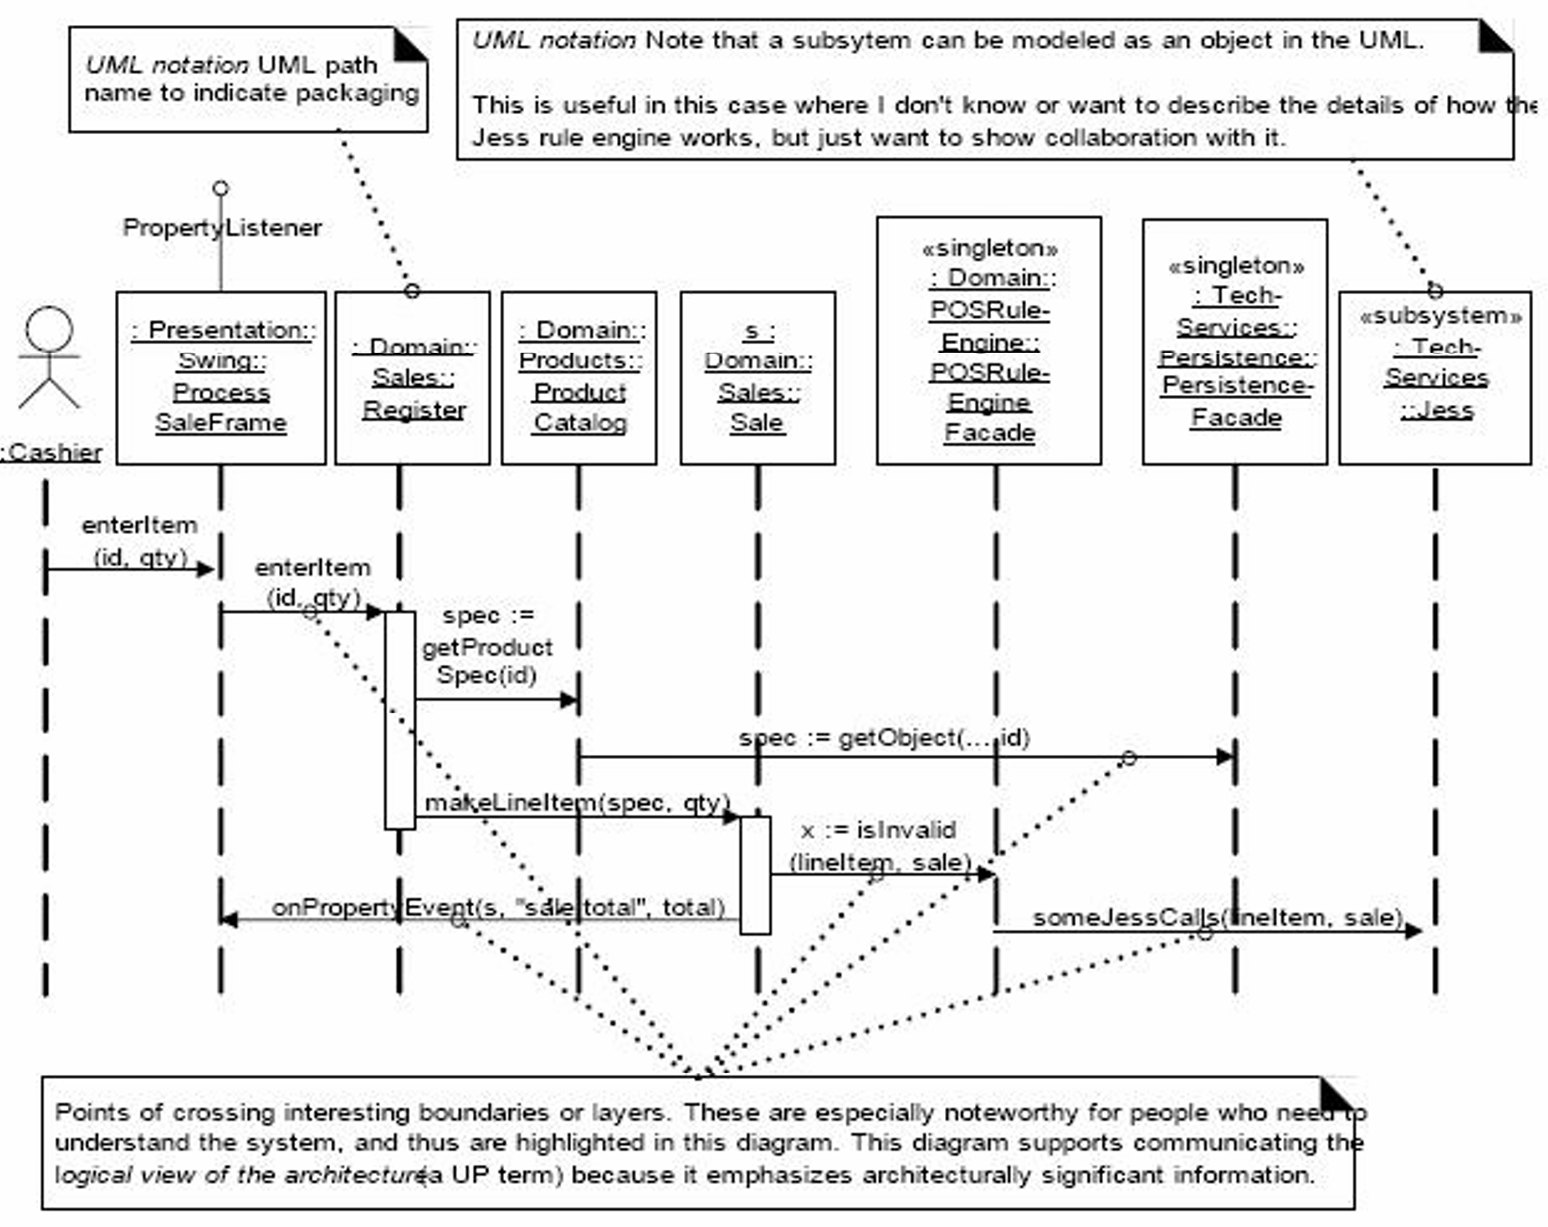
\includegraphics[scale=0.23]{architettura_layer/diagramma_sequenza.png}
    \end{center}
    \newpage
    \noindent Nel diagramma si possono fare delle considerazioni:
    \begin{enumerate}
        \item In UML si può illustrare il nome del package a cui una certa classe appartiene con la seguente dicitura: \textit{<PackageName>::<TypeName>}.
              Ciò permette di evidenziare le connessioni fra package e layer all'interno di un diagramma dinamico.
        \item Lo sterotipo \textit{<<subsystem>>} indica un'entità con il suo comportamento e le sue interfacce. Può essere modellato da un package
              o da un oggetto.
        \item Il diagramma di sequenza mostra solo le relazioni rilevanti dal punto di vista architetturale.
    \end{enumerate}
    Bisogna precisare che alcuni package rappresentano veri e propri sottosistemi indipendenti (stereotipi),
    con il proprio comportamento e le loro interfacce. Altri package \textbf{NON} sono sottosistemi.

    \mysubsubsectionformatted{Collaborazione tra pattern Layers e design pattern}
    Come detto prima, il pattern architetturale serve per definire le parti più grandi del sistema. Per poter stabilire le
    connessioni tra gli stati e i package verranno usati i design pattern. Spesso sono usati il \textbf{Facade}, \textbf{Observer},
    e \textbf{Controller}, quindi i pattern GRASP.

    \mysubsubsectionformatted{Funzionamento del Facade}
    Viene utilizzato per accedere alle funzionalità offerte da un sottosistema. Facade permette di nascondere il sottosistema dietro un'interfaccia
    unificata. Facade non espone le operazioni di basso livello, ma quelle di alto livello utilizzabili dai client.
    \begin{center}
        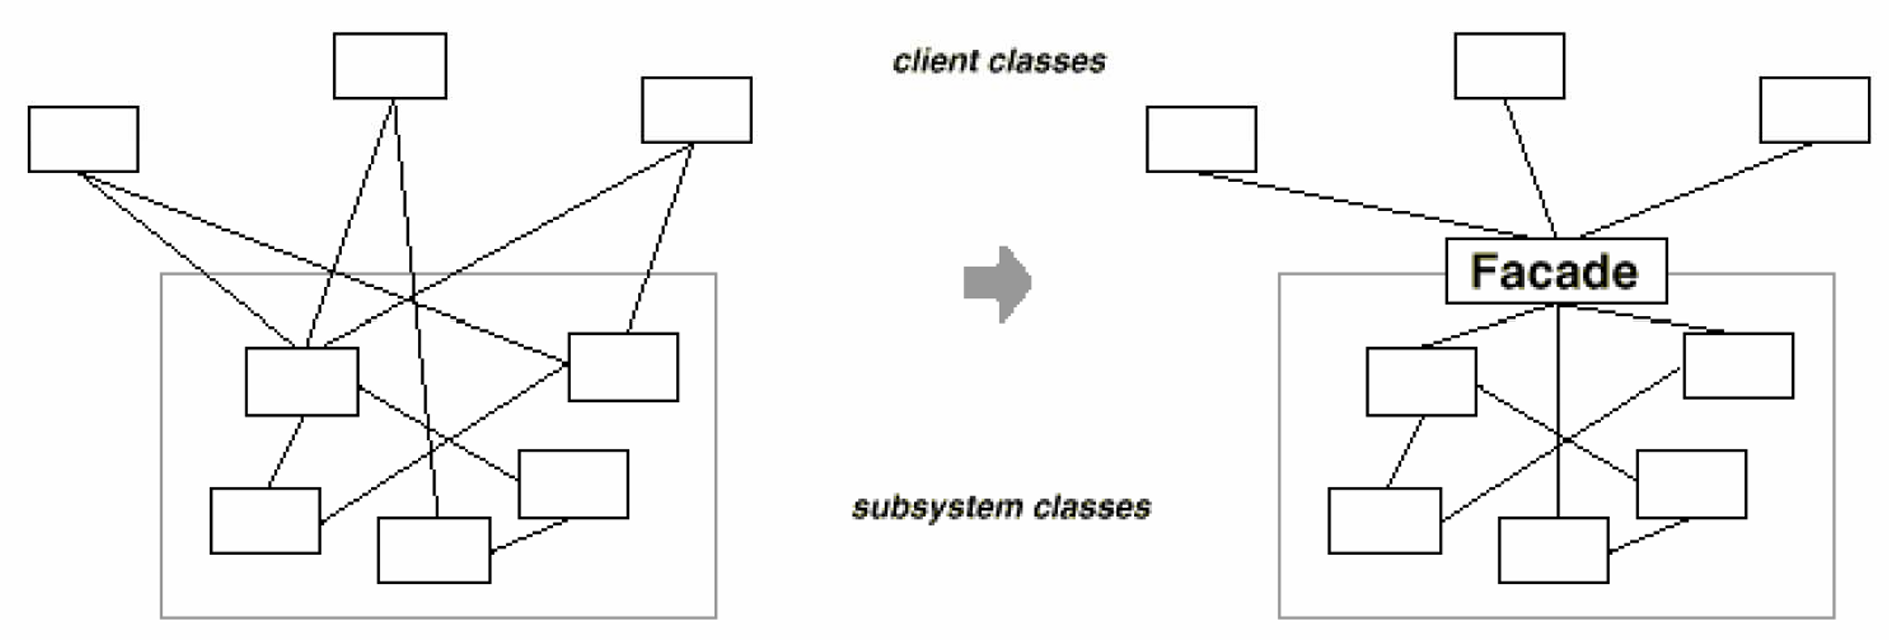
\includegraphics[scale=0.25]{architettura_layer/facade.png}
    \end{center}
    \newpage
    \mysubsubsectionformatted{Funzionamento del Controller}
    Viene utilizzato per descrivere le scelte comuni tipiche degli handler lato client per le richieste di operazioni di sistema provenienti
    dal Presentation Layer (UI).
    \begin{center}
        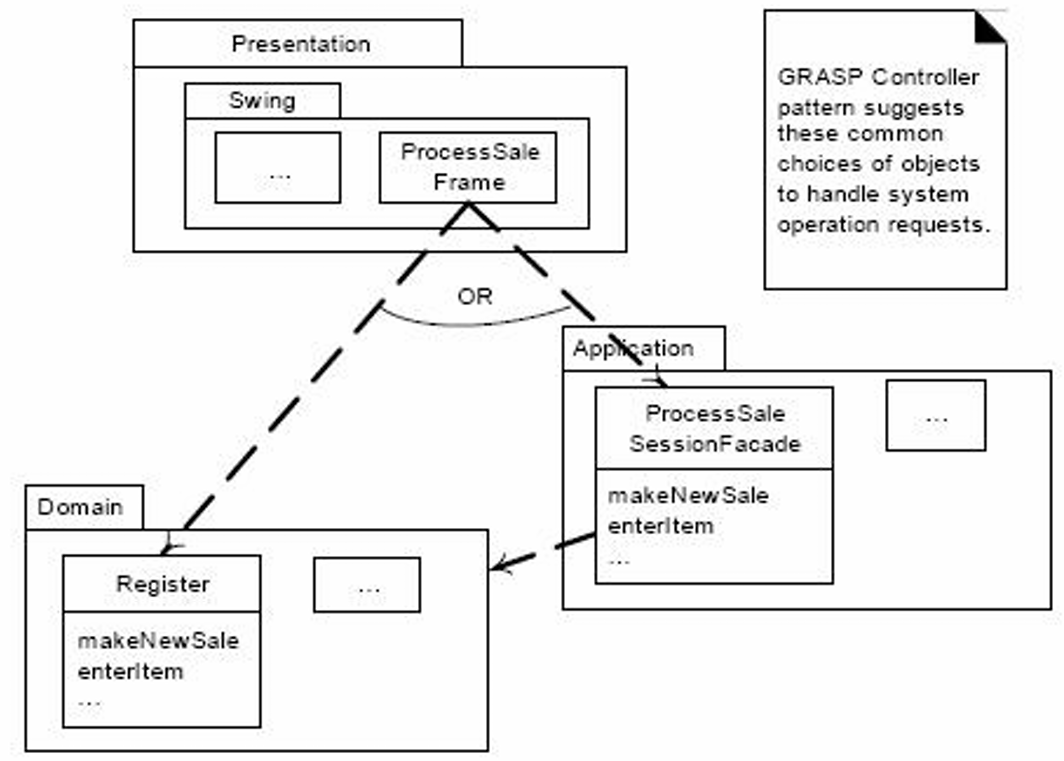
\includegraphics[scale=0.32]{architettura_layer/controller.png}
    \end{center}
    Si tratta quindi del primo oggetto oltre lo stato UI che coordina le operazioni di sistema, in grado di ricevere e gestire un messaggio di un'operazione
    di sistema. Quando si parla di operazioni di sistema si intendono gli eventi di input principali del sistema.
    \\
    Tra i vantaggi del Controller abbiamo:
    \begin{enumerate}
        \item Logica applicativa non gestita nello strato di interfaccia.
        \item Riuso della logica.
        \item Si possono usare interfacce diverse.
    \end{enumerate}
    Quando si usano i Controller, accade di compiere l'errore di "gonfiarlo":
    \begin{itemize}
        \item Un solo Controller riceve numerosi eventi di sistema.
        \item Il Controller svolge parte del lavoro prima di delegarlo.
        \item Il Controller ha numerosi attributi e conserva le informazioni sul sistema e sul dominio.
    \end{itemize}
    \newpage
    
    \noindent Un modo per vedere le operazioni di sistema è tramite i \textbf{Diagrammi di Interazione}.
    \begin{center}
        \includegraphics[scale=0.28]{architettura_layer/diagramma_attività.png}
    \end{center}

    \mysubsubsectionformatted{Funzionamento di Observer}
    Ipotizzando che il layer Application o Domain debbano comunicare con il Presentation, l'Observer è utile al caso.
    \\
    Questo design pattern permette di notificare e aggiornare automaticamente tutti gli oggetti dipendenti da un'oggetto 'padre'
    che prende il nome di Subject.
    \begin{center}
        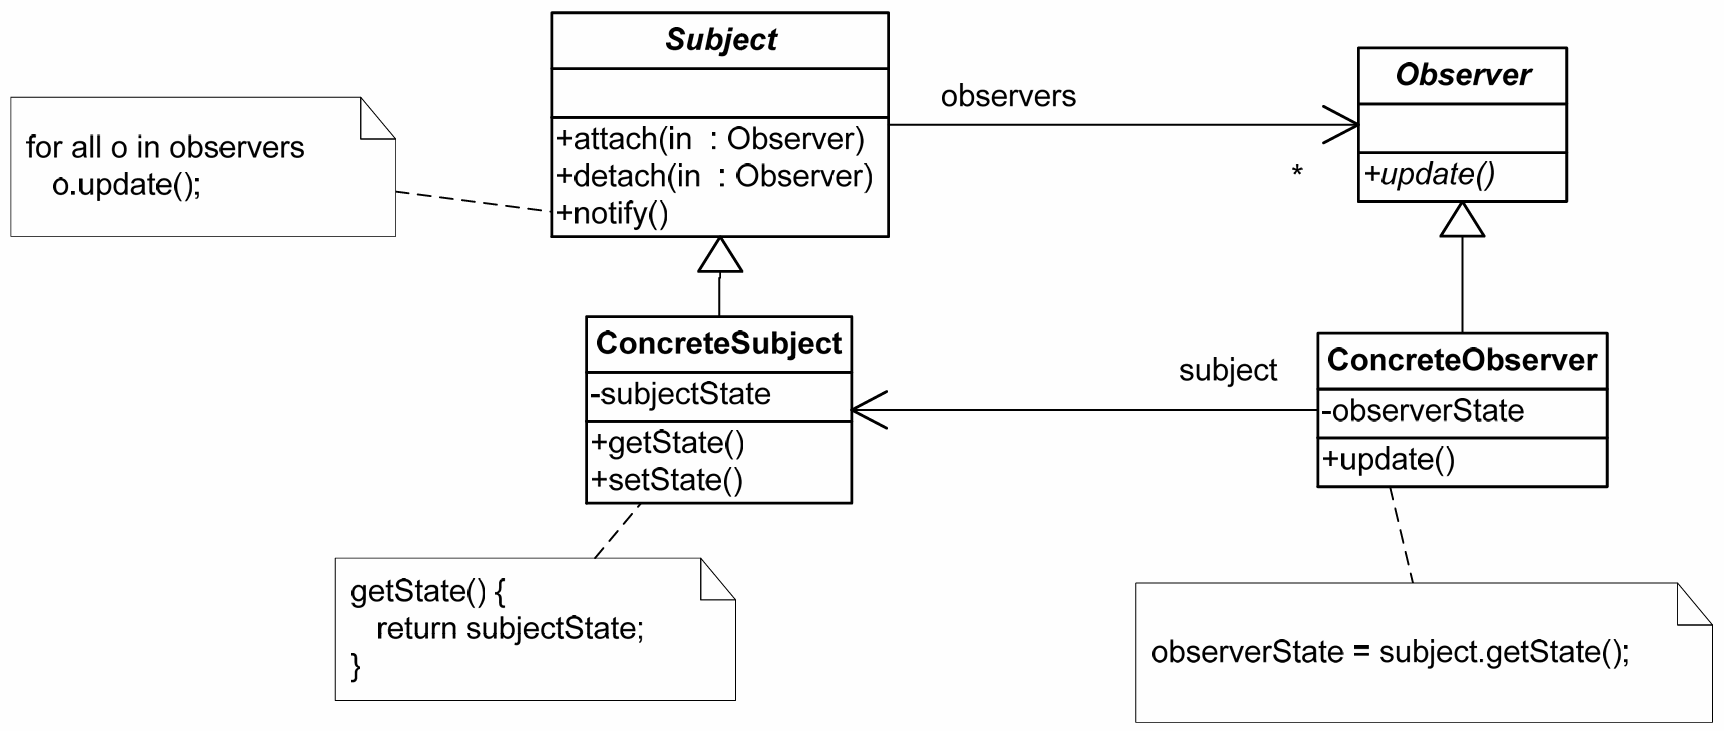
\includegraphics[scale=0.27]{architettura_layer/observer.png}
    \end{center}
    \newpage
}